% !TEX encoding = UTF-8
% !TEX TS-program = pdflatex
% !TEX root = ../tesi.tex
% !TEX spellcheck = it-IT

%************************************************
\chapter{Classificazione}
\label{cap:ctbnc}
%************************************************
La classificazione è un argomento centrale nei campi di ricerca relativi all'apprendimento automatico e l'analisi dei dati. In generale, essa consiste nel processo di assegnare una \emph{classe} (\ie{} un'etichetta) a delle istanze descritte da un insieme di attributi. Si parla di \emph{classificazione supervisionata} quando è necessario indurre un classificatore a partire da un insieme di dati composto da istanze già etichettate e utilizzare tale classificatore per classificare nuove istanze di dati.

In questo capitolo viene quindi introdotta una classe di modelli, che prende il nome di \acf{CTBNC}, il cui scopo è la \emph{classificazione supervisionata} di traiettorie multivariate di variabili discrete a \emph{tempo continuo}. Si descrivono due istanze di tale classe: i classificatori \acf{CTNB} e i classificatori \acf{CTTANB}; classificatori per i quali si affronta il processo di apprendimento in caso di dati completi.

Infine, nella \autoref{sec:inference-ctbnc}, si presenta un algoritmo di inferenza esatta per la classe dei \acs{CTBNC}.

\section{Classificatore}\label{sec:ctbnc}
Al fine di risolvere il succitato problema della classificazione sono stati proposti numerosi approcci. Ad esempio, \citet{DudaHart1973} e \citet{Langley1992} hanno proposto uno dei classificatori più performanti, il \lwcase \nb{} \class{}.

Il modello definito dalle \acl{CTBN} (\myref[si veda la definizione]{defn:ctbn}), come mostrato in~\citet{Stella2012}, può essere utilizzato al fine di costruire un modello di \emph{classificazione supervisionata} che rappresenta l'evoluzione nel tempo continuo di una variabile di processo $\set{X}$ (\ie{} insieme di \mprocess{}, \myref[si veda la definizione]{defn:pv}).

Al fine di costruire questa nuova classe di modelli di classificazione supervisionata è necessario un nodo aggiuntivo associato alla classe $\setel{Y}$.
\begin{definizione}[\acl{CTBNC}]\label{defn:ctbnc}
Un \acf{CTBNC} è composto da una coppia $\conceptsym{C}=(\conceptsym{N}\,,\,\set{P}(\setel{Y}))$ dove:
\begin{itemize}
    \item $\conceptsym{N}$ è una \acs{CTBN} con nodi attributo $\setel{X_1}\,,\,\setel{X_2}\,,\,\dotsc\,,\,\setel{X_N}$
    \item $\setel{Y}$ è il nodo classe con valori $val(\setel{Y})=\{\,\vectel{y_1}\,,\,\dotsc\,,\,\vectel{y_K}\,\}$ e probabilità marginale $\set{P}(\setel{Y})$.
\end{itemize}
E inoltre il grafo su $\conceptsym{N}$ (\ie{} il grafo $\conceptsym{G}$, \myref[si veda la definizione]{defn:ctbn}) rispetta le seguenti condizioni:
\begin{itemize}
    \item $\conceptsym{G}$ è un grafo connesso\footnote{Il grafo $\conceptsym{G} = (\setel{V}, \setel{E})$ è detto \emph{connesso} se $\forall \: (\setel{u}\,,\,\setel{v}) \in \setel{V}$ esiste un cammino che collega $\setel{u}$ a $\setel{v}$.}
    \item $Pa(\setel{Y})=\{\,\}$, \ie{} la variabile casuale $\setel{Y}$ è associata a un nodo radice\footnote{In un grafo un nodo è detto \emph{radice} qualora esso non abbia alcun genitore.}
    \item il nodo $\setel{Y}$ è indipendente dal tempo ed è specificato solo ed esclusivamente dalla sua probabilità marginale $\set{P}(\setel{Y})$.
\end{itemize}
\end{definizione}
A supporto della \myref[definizione]{defn:ctbnc}, la figura~\vref{fig:ctbnc-example} fornisce un'istanza di \acs{CTBNC} composta dai nodi attributi $\setel{X_1},\setel{X_2},\setel{X_3},\setel{X_4},\setel{X_5}$ e dal nodo classe $\setel{Y}$ (nodo radice). Si osservi come tale istanza contenga dei cicli, uno riguardante i nodi $\setel{X_2},\setel{X_4},\setel{X_5},\setel{X_3}$ e l'altro riguardante i nodi $\setel{X_1},\setel{X_3}$.

\begin{figure}
\centering
\includegraphics[width=0.9\columnwidth]{immagini/ctbnc}
\caption[Un esempio di \acs{CTBNC}]{Un esempio di \acf{CTBNC} con cinque nodi attributo, $\setel{X}_1\,,\,\dotsc\,,\,\setel{X}_5$, e un nodo classe, $\setel{Y}$.}
\label{fig:ctbnc-example}
\end{figure}

% TODO: quali motivazioni?
Seguendo le stesse motivazioni che hanno portato~\citet{Friedman1997} a sfruttare il modello delle \acl{BN} per costruire un \acf{BNC} e successivamente estendere questo modello di classificazione supervisionata imponendovi una struttura ad albero, creando un \acf{TAN} \class{}, si presentano di seguito due istanze di classificatori appartenenti alla classe dei \acf{CTBNC}: il \acf{CTNBC} e il \acf{CTTANBC}.

\begin{definizione}[\acl{CTNBC}]\label{defn:ctnbc}
Un \acf{CTNBC} è un \acl{CTBNC} $\conceptsym{C}=(\conceptsym{N}\,,\,\set{P}(\setel{Y}))$ caratterizzato dal fatto che ogni nodo attributo ha un solo genitore, il nodo classe $\setel{Y}$. Risulta quindi che:
\[
Pa(\setel{X}_i)=\{\,\setel{Y}\,\} \quad \forall \; \setel{X}_i \in \conceptsym{G}\text{.}
\]
\end{definizione}
Come mostrato dalla figura~\vref{fig:ctnb}, un \acs{CTNBC} possiede un nodo radice, associato alla variabile casuale $\setel{Y}$, che è l'unico genitore di tutti i restanti nodi $\setel{X}_i$, con $i=1,2,\,\dotsc\,,N$, che lo compongono.

% TODO: commentare circa la struttura e le assunzioni che codifica: e.g indipendenza condizionale [ QUESTO SOPRA, modificato un po' e sintetizzato]
% One of the most effective classifiers, in the sense that its predictive performance is competitive with state-of-the-art classifiers, is the so-called naive Bayesian classifier described, for example, by Duda and Hart (1973) and by Langley et al. (1992). This classifier learns from training data the conditional probability of each attribute Ai given the class label C. Classification is then done by applying Bayes rule to compute the probability of C given the particular instance of A1,...,An, and then predicting the class with the highest poste- rior probability. This computation is rendered feasible by making a strong independence assumption: all the attributes Ai are conditionally independent given the value of the class C. By independence we mean probabilistic independence, that is, A is independent of B given C whenever Pr(A|B,C) = Pr(A|C) for all possible values of A,B andC, whenever Pr(C) > 0.
% The performance of naive Bayes is somewhat surprising, since the above assumption is clearly unrealistic. Consider, for example, a classifier for assessing the risk in loan applications: it seems counterintuitive to ignore the correlations between age, education level, and income. This example raises the following question: can we improve the performance of naive Bayesian classifiers by avoiding unwarranted (by the data) assumptions about independence? In order to tackle this problem effectively, we need an appropriate language and efficient machinery to represent and manipulate independence assertions. Both are provided by Bayesian networks (Pearl, 1988) [link a definizione/sezione ad esse riguardante]

% When represented as a Bayesian network, a naive Bayesian classifier has the simple structure depicted in Figure 1. This network captures the main assumption behind the naive Bayesian classifier, namely, that every attribute (every leaf in the network) is independent from the rest of the attributes, given the state of the class variable (the root in the network).
% Since we have the means to represent and manipulate independence assertions, the obvious question follows: can we induce better classifiers by learning unrestricted Bayesian networks?

% TODO: si noti che qui gli archi rappresentano dipendenze causali nel tempo.

\begin{figure}
\centering
\includegraphics[width=0.9\columnwidth]{immagini/ctnb}
\caption[Un \acs{CTNBC}]{Un \acf{CTNBC}.}
\label{fig:ctnb}
\end{figure}

\begin{definizione}[\acl{CTTANBC}]\label{defn:cttanbc}
Un \acf{CTTANBC} è un \acl{CTBNC} $\conceptsym{C}=(\conceptsym{N}\,,\,\set{P}(\setel{Y}))$ che rispetta i seguenti vincoli:
\begin{itemize}
    \item $\setel{Y} \in Pa(\setel{X}_i)$ con $i=1,2,\,\dotsc\,,N$
    \item i nodi attributo $\setel{X}_i$, $i=1,2,\,\dotsc\,,N$, formano un albero:
    \[
    \exists \; j \; : \quad |Pa(\setel{X}_j)|=1 \quad \text{mentre per} \quad i \neq j \; : \quad |Pa(\setel{X}_i)|=2\text{.}
    \]
\end{itemize}
\end{definizione}

% TODO: esempio sulla "rimozione" del nosto Y .. albero formato da .. (collegarsi dall'immagine)
% TODO: dire che è una estensione (o riduzione, dati i vincoli ulteriori) del CTNBC (e far notare che differisce solo nel fatto che i nodi figli nel nodo classe hanno archi tra di loro, o più semplicemente che la cardinalità degli insieme Pa dei nodi attributo non è sempre pari a 1)

\section{Apprendimento}\label{sec:learning-ctbnc}
...

% TODO: partire di qua? come mostra la figura d'esempio 1 bla bla
% Several considerations concerning the exploitation of the structure of the graph G of the CTBNC in the case where the classification task is performed on a fully observed J-evidence-stream can be made. In such an evidential setting, the only unobserved random variable is the class variable Y; thus it is possible to fruitfully and conditionally exploit independence relationships between random variables as it happens in ordinary BNs

\begin{figure}
\centering
\includegraphics[width=0.9\columnwidth]{immagini/cttanb}
\caption[Un \acs{CTTANBC}]{Un \acf{CTTANBC}: qualora la variabile classe $\setel{Y}$ venga rimossa, le variabili rimanenti formano un albero.}
\label{fig:cttanb}
\end{figure}

\section{Inferenza}\label{sec:inference-ctbnc}
...

\subsection{Na\"ive Bayes}\label{sec:inference-ctnb}
...

% TODO
% They implement a trade-off between computational complexity and classification accuracy.
% The performance of the continuous time naive Bayes classifier is assessed in the case where real-time feedback to neurological patients undergoing motor rehabilitation must be provided
